\documentclass[12pt]{ucsddissertation}
% mathptmx is a Times Roman look-alike (don't use the times package)
% It isn't clear if Times is required. The OGS manual lists several
% "standard fonts" but never says they need to be used.
%\usepackage{mathptmx}

\usepackage{fontspec}
\setmainfont{Times New Roman}
\setmonofont{DejaVuSansMono}
%\renewcommand{\familydefault}{\sfdefault}
%\usepackage[scaled=1]{helvet}

\usepackage[NoDate]{currvita}
\usepackage{array}
\usepackage{tabularx}
\usepackage{booktabs}
\usepackage{ragged2e}
\usepackage{microtype}
\usepackage[breaklinks=true,pdfborder={0 0 0}]{hyperref}
\usepackage{graphicx}

% Valentin
\usepackage[english]{babel}
\usepackage{DejaVuSansMono}
\let\textlozenge\relax
%\usepackage{gfsdidot}
\usepackage{minted}
\usepackage[parfill]{parskip}

\AtBeginDocument{%
	\settowidth\cvlabelwidth{\cvlabelfont 0000--0000}%
}

\setminted{
  linenos=true,
  breaklines=true,
  encoding=utf8,
  fontsize=\footnotesize,
  frame=lines
}
\AtBeginEnvironment{minted}{\dontdofcolorbox}
\def\dontdofcolorbox{\renewcommand\fcolorbox[4][]{##4}}

% OGS recommends increasing the margins slightly.
\increasemargins{.1in}

% These are just for testing/examples, delete them
\usepackage{trace}
%\usepackage{showframe} % This package was just to see page margins
\usepackage[english]{babel}
\usepackage{blindtext}
\overfullrule5pt
% ---

% Required information
\title{This is the Title of My Dissertation}
\author{Valentin Robert}
\degree{Computer Science}{Doctor of Philosophy}
% Each member of the committee should be listed as Professor Foo Bar.
% If Professor is not the correct title for one, then titles should be
% omitted entirely.
\chair{Professor Sorin Lerner}
%\cochair{Professor Gamma Delta} % Optional
% Your committee members (other than the chairs) must be in alphabetical order
\committee{Professor William Griswold}
\committee{Professor Ranjit Jhala}
\committee{Professor James Hollan}
\committee{Professor Todd Millstein}
\degreeyear{2018}

%%%%% General-purpose text macros %%%%%
\newcommand{\define}[1]{\emph{#1}}
\newcommand{\mycite}[1]{\citeauthor{#1}~\cite{#1}}

\newcommand{\Language}[1]{\emph{#1}}
\newcommand{\Tool}[1]{\emph{#1}}
\newcommand{\Gallina}{\Language{Gallina}}
\newcommand{\Ltac}{\Language{Ltac}}
\newcommand{\Vernacular}{\Language{Vernacular}}

\newcommand{\Chick}{\Language{Chick}}
\newcommand{\Coq}{\Language{Coq}}
\newcommand{\CoqIDE}{\Tool{CoqIDE}}
\newcommand{\Haskell}{\Language{Haskell}}
\newcommand{\JavaScript}{\Language{JavaScript}}
\newcommand{\OCaml}{\Language{OCaml}}
\newcommand{\PeaCoq}{\Language{PeaCoq}}
\newcommand{\RxJS}{\Language{RxJS}}
\newcommand{\SerAPI}{\Tool{SerAPI}}
\newcommand{\Snap}{\Language{Snap}}
\newcommand{\TypeScript}{\Language{TypeScript}}

\newcommand{\OperatorColor}{purple}
\newcommand{\Operator}[1]{\textcolor{\OperatorColor}{\ #1\ }}
\newcommand{\Entails}{\Operator{\vdash}}
\newcommand{\HasType}{\Operator{:}}

%\newmintinline{coq}{fontsize=\small}
% \newcommand{\coqinline}[1]{%
%   %\colorbox{monokaibg}{%
%   \parbox[c][0.9em]{\widthof{\mycoq{#1}}}{\mycoq{#1}}%
%   %}%
% }

\newcommand{\modified}[1]{\color{Orange}{#1}}
\newcommand{\repaired}[1]{\color{PineGreen}{#1}}

\newcommand{\rulename}[1]{$\LeftTirNameStyle{#1}$}

\newcommand{\RmApp}{Rm-App}
\newcommand{\RmPi}{Rm-Pi}
\newcommand{\InsApp}{Ins-App}

%%%%% Math-mode macros %%%%%

\newcommand{\opcolor}{purple}
\newcommand{\out}[1]{ \boxed{ \textcolor{teal}{#1} } }
\newcommand{\MathPatches}[3]{%
#1 \overset{#2}{\mathbin{\textcolor{\opcolor}{\rightsquigarrow}}} \out{#3}%
}

\newcommand{\App}{\$}
\newcommand{\Mod}{Mod}
\newcommand{\Drop}{Drop}
\newcommand{\Ins}{Ins}
\newcommand{\Keep}{Keep}
\newcommand{\Lam}{\lambda}

\newcommand{\oMod}{\overset{\mathtt{\Mod}}}
\newcommand{\oDrop}{\overset{\mathtt{\Drop}}}
\newcommand{\oIns}{\overset{\mathtt{\Ins}}}
\newcommand{\oKeep}{\overset{\mathtt{\Keep}}}

\newcommand{\Cons}{::}
\newcommand{\permute}[2]{%
\overline{#2}^{\overset{#1}{\rightleftarrows}}%
}
\newcommand{\permuteOp}[2]{%
\overset{\overset{#1}{\rightleftarrows}}{#2}%
}

\newcommand{\mkMathPiRaw}[4]{#3{\Pi} #4{#1} \rightarrow #2}
\newcommand{\mkMathPi}[5]{\mkMathPiRaw{(#2 : #1)}{#3}{#4}{#5}}


\newcommand{\MathCons}[2]{#1 \Cons #2}
\newcommand{\MathDrop}[1]{\oDrop{\Cons} #1}
\newcommand{\MathDropApp}[1]{\oDrop{\App} #1}
\newcommand{\MathDropLam}[1]{\oDrop{\Lam} #1}
\newcommand{\MathDropPi}[1]{\oDrop{\Pi} #1}
\newcommand{\MathHole}{\texttt{\_}}
\newcommand{\MathIns}[2]{#1 \oIns{\Cons} #2}
\newcommand{\MathInsApp}[2]{\mkMathApp{#1}{#2}{\oIns}}
\newcommand{\MathInsAppOp}{\oIns{\App}}
\newcommand{\MathInsLam}[2]{\mkMathLam{#1}{#2}{\oIns}{}}
\newcommand{\MathInsLamOp}{\oIns{\Lam}}
\newcommand{\MathInsPi}[3]{\mkMathPi {#1}{#2}{#3}{\oIns}{}}
\newcommand{\MathInsPiOp}{\oIns{\Pi}}
\newcommand{\MathLam}[2]{\mkMathLam{#1}{#2}{}{}}
\newcommand{\MathLams}[3]{\mkMathLam{#1}{#2}{}{\BarCount{#3}}}
\newcommand{\MathKeepPiOp}{\oKeep{\Pi}}
\newcommand{\MathMod}[2]{#1 \oMod{\Cons} #2}
\newcommand{\MathModAppOp}{\oMod{\App}}
\newcommand{\MathModLamOp}{\oMod{\Lam}}
\newcommand{\MathModPiOp}{\oMod{\Pi}}
\newcommand{\MathPermute}[2]{\permuteOp{#1}{\Cons} #2}
\newcommand{\MathPermuteLams}[2]{\permuteOp{#1}{\lambda} #2}
\newcommand{\MathPermutePis}[2]{\permuteOp{#1}{\Pi} #2}
\newcommand{\MathPi}[3]{\mkMathPi{#1}{#2}{#3}{}{}}
\newcommand{\MathPis}[4]{\mkMathPi{#1}{#2}{#3}{}{\BarCount{#4}}}
\newcommand{\MathReplace}[1]{\mathds{K}({#1})}
\newcommand{\MathSame}{\mathds{1}}

\newcommand{\mkMathApp}[3]{#1 #3{ \$ } #2}

%%% REPAIR %%%

\newcommand{\op}[1]{\textcolor{\opcolor}{#1}}

\newcommand{\boundOp}{\op{\text{Bound}}}
\newcommand{\freshOneOp}{\op{\text{Fresh}_1}}
\newcommand{\freshTwoOp}{\op{\text{Fresh}_2}}
\newcommand{\repairIndOp}{\op{R_{I}}}
\newcommand{\repairProgOp}{\op{R_{P}}}
\newcommand{\repairTermOneOp}{\op{R_{T_1}}}
\newcommand{\repairTermTwoOp}{\op{R_{T_2}}}
\newcommand{\repairTermThreeOp}{\op{R_{T_2}}}
\newcommand{\repairVernacOp}{\op{R_{V}}}
\newcommand{\vernacEnvOp}{\op{E_{V}}}
\newcommand{\repairBranchesOp}{\op{R_{B}}}

\newcommand{\blackbrackets}[1]{\left[ #1 \right]}
\newcommand{\blackdiff}[2]{\blackbrackets{\genfrac{}{}{0pt}{}{#1}{#2}}}
\newcommand{\bound}[1]{\boundOp\op{(}#1\op{)}}
\newcommand{\brackets}[1]{%
  \color{\opcolor} \left[ \normalcolor #1 \color{\opcolor} \right] \normalcolor%
}
\newcommand{\context}[2]{#1 \op{,} #2}
\newcommand{\dcontext}[4]{\context{\diff{#1}{#2}}{\diff{#3}{#4}}}
\newcommand{\denv}[2]{\diff{#1}{#2}}
\newcommand{\diff}[2]{\brackets{\genfrac{}{}{0pt}{}{#1}{#2}}}
\newcommand{\dtau}[1]{\delta_{\tau_{#1}}}
\newcommand{\equals}[2]{#1 \mathbin{\textcolor{\opcolor}{=}} #2}
\newcommand{\freshOne}[3]{\freshOneOp\op{(}\diff{#1}{#2}\op{) =}\ \out{#3}}
\newcommand{\freshTwo}[3]{\freshTwoOp\op{(}#1\op{,}#2\op{) =}\ \out{#3}}
\newcommand{\genericrepair}[3]{\mkrepair{\repairTermTwoOp}{#1}{#2}{#3}{\op{?}}}
\newcommand{\nturnstile}[2]{#1 \mathbin{\textcolor{\opcolor}{\nvdash}} #2}
\newcommand{\qmark}{\textcolor{\opcolor}{?}}
\newcommand{\squiggly}[2]{#1 \mathbin{\textcolor{\opcolor}{\rightsquigarrow}} #2}
\newcommand{\subst}[2]{#1 \leftarrow #2}
\newcommand{\turnstile}[2]{#1\ \mathbin{\textcolor{\opcolor}{\vdash}}\ #2}
\newcommand{\repair}[4]{ \mkrepair{\repairTermOneOp}{#1}{#2}{#3}{#4} }
\newcommand{\repairBranches}[3]{\mksimplerepair{\repairBranchesOp}{#1\op{,}\ #2}{#3}}
\newcommand{\repairInd}[7]{
  \mksimplerepair%
  {\repairIndOp}
  {\diff{#1}{#2}\op{,}\ \diff{#3}{#4}\op{,}\ \diff{#5}{#6}}
  {#7}
}
\newcommand{\repairProg}[3]{
  \repairProgOp\op{(}\blackdiff{#1}{#2}\op{)}\ \op{=}\ \out{#3}
}
\newcommand{\repairTerm}[4]{\mkrepair{\repairTermOneOp}{#1}{#2}{#3}{#4}}
\newcommand{\repairTermWithoutType}[2]{\mksimplerepair{\repairTermThreeOp}{#1}{#2}}
\newcommand{\repairVernac}[3]{
  \repairVernacOp\op{(}\blackdiff{#1}{#2}\op{)}\ \op{=}\ \out{#3}
}

\newcommand{\DefinitionText}{\text{Definition}}
\newcommand{\InductiveText}{\text{Inductive}}
\newcommand{\ConstructorText}{\text{Constructor}}
\newcommand{\GlobalDefinitionText}{\text{GlobalDefinition}}
\newcommand{\GlobalInductiveText}{\text{GlobalInductive}}

\newcommand{\Definition}[4]{ \DefinitionText(\{ #1, #2, #3, #4 \}) }
\newcommand{\Inductive}[5]{ \InductiveText(\{ #1, #2, #3, #4, #5 \}) }
\newcommand{\Constructor}[3]{ \ConstructorText(\{ #1, #2, #3 \}) }
\newcommand{\GlobalDefinition}[3]{ \GlobalDefinitionText(\{ #1, #2, #3 \}) }
\newcommand{\GlobalInductive}[5]{ \GlobalInductiveText(\{ #1, #2, #3, #4, #5 \}) }

\newcommand{\ModifyDefinition}[4]{ \delta_{\DefinitionText}(\{ #1, #2, #3, #4 \}) }
\newcommand{\ModifyInductive}[5]{ \delta_{\InductiveText}(\{ #1, #2, #3, #4, #5 \}) }
\newcommand{\ModifyGlobalDefinition}[3]{ \delta_{\GlobalDefinitionText}(\{ #1, #2, #3 \}) }
\newcommand{\ModifyGlobalInductive}[5]{ \delta_{\GlobalInductiveText}(\{ #1, #2, #3, #4, #5 \}) }

\newcommand{\GlobalDefinitionAnon}{\GlobalDefinitionText(\{ \ldots \})}
\newcommand{\GlobalInductiveAnon}{\GlobalInductiveText(\{ \ldots \})}

\newcommand{\DefinitionAnon}{\DefinitionText(\{ \ldots \})}
\newcommand{\InductiveAnon}{\InductiveText(\{ \ldots \})}

\newcommand{\RepairProg}[1]{R-Prog-#1}

\newcommand{\RProgMod}{\RepairProg{Modify}}
\newcommand{\RProgKeep}{\RepairProg{Keep}}
\newcommand{\RProgSameCons}{\RepairProg{Same-Cons}}

\newcommand{\scalefactor}{1}
\newcommand{\invscalefactor}{1}

\NewEnviron
    {Rules}[2]
    {
      \begin{figure*}
        %\scalebox{\invscalefactor}{
          %\begin{minipage}{\scalefactor\textwidth}
            %\begin{mathpar}
              \BODY
            %\end{mathpar}
          %\end{minipage}
        %}
        \caption{#2}
        \label{#1}
      \end{figure*}
    }

\newcommand{\MathSameProg}{\MathSame_P}
\newcommand{\MathSameVernac}{\MathSame_V}
\newcommand{\MathSameGlobal}{\MathSame_G}

\newcommand{\MathProp}{\mathtt{Prop}}
\newcommand{\MathSet} {\mathtt{Set}}
\newcommand{\MathType}{\mathtt{Type}}

\newcommand{\hasType}[2]{ #1\ \op{:}\ #2 }

\newcommand{\mkrepair}[5]{
  #1
  \op{(}
  \hasType
  { #2 }
  { \diff{ #4 }{ #5 } }
  \op{) =\ }
  \out{ #3 }
}

\newcommand{\MathLocalAssum}[2]{ ( #1 : #2 ) }
\newcommand{\MathLocalDef}[3]{ ( #1 : #2 \coloneqq #3 ) }

\newcommand{\mksimplerepair}[3]{
  #1
  \op{(}
  #2
  \op{) =\ }
  \out{ #3 }
}

\newcommand{\RModPi}{\RepairTerm{Mod-$\Pi$}}
\newcommand{\RInsPi}{\RepairTerm{Ins-$\Pi$}}
\newcommand{\RDropPi}{\RepairTerm{Drop-$\Pi$}}
\newcommand{\RPermutePis}{\RepairTerm{Permute-$\Pi$s}}
\newcommand{\RReplace}{\RepairTerm{Replace}}
\newcommand{\RSame}{\RepairTerm{$\MathSame{}$-Other}}
\newcommand{\RSamePi}{\RepairTerm{$\MathSame{}$-$\Pi$}}

\newcommand{\RepairTermPrefix}{RT1}
\newcommand{\GenericRepairPrefix}{R-Term-2}
\newcommand{\UnknownTypeRepairPrefix}{R-Term-2}

\newcommand{\RepairTerm}[1]{\RepairTermPrefix-#1}
\newcommand{\GenericRepair}[1]{\GenericRepairPrefix-#1}
\newcommand{\UnknownTypeRepair}[1]{\UnknownTypeRepairPrefix-#1}

\newcommand{\mkMathLam}[4]{#3{\lambda} #4{#1} \rightarrow #2}

\newcommand{\MathModApp}[2]{ \mkMathApp{#1}{#2}{\oMod}{} }
\newcommand{\MathModLam}[2]{ \mkMathLam{#1}{#2}{\oMod}{} }
\newcommand{\MathModPi} [3]{ \mkMathPi{#1}{#2}{#3}{\oMod}{} }
\newcommand{\MathKeepPi}[1]{ \MathKeepPiOp \rightarrow #1 }

\newcommand{\MathAnnot}[2]{#1 : #2}

\newcommand{\UTRApp}{\UnknownTypeRepair{App}}
\newcommand{\UTRMatch}{\UnknownTypeRepair{Match}}
\newcommand{\UTRPi}{\UnknownTypeRepair{Pi}}
\newcommand{\UTRType}{\UnknownTypeRepair{Universe}}
\newcommand{\UTRVar}{\UnknownTypeRepair{Var}}
\newcommand{\UTRAnnot}{\UnknownTypeRepair{Annot}}
\newcommand{\UTRHole}{\UnknownTypeRepair{Hole}}
\newcommand{\UTROtherwise}{\UnknownTypeRepair{Otherwise}}

\newcommand{\repairArgsOp}{\op{R_{Fn}}}

\newcommand{\repairArgs}[5]{
  \op{\repairArgsOp(}#1\op{,} #2\op{,} #3\op{,} #4\op{) =}\ \out{#5}
}

\newcommand{\declDiff}[3]{
  \hasType
      { \diff{ #1 }{ \out{#2} } }
      { \diff{ \op{?} }{ \out{#3} } }
}

\newcommand{\MathMatch}[2]{ \text{match}\ #1\ \text{with}\ #2 }


% Start the document
\begin{document}
% Begin with frontmatter and so forth
\frontmatter
\maketitle
\makecopyright
\makesignature
% Optional
% \begin{dedication}
% \setsinglespacing
% \raggedright % It would be better to use \RaggedRight from ragged2e
% \parindent0pt\parskip\baselineskip
% In recognition of reading this manual before beginning to format the
% doctoral dissertation or master's thesis; for following the
% instructions written herein; for consulting with OGS Academic Affairs
% Advisers; and for not relying on other completed manuscripts, this
% manual is dedicated to all graduate students about to complete the
% doctoral dissertation or master's thesis.

% In recognition that this is my one chance to use whichever
% justification, spacing, writing style, text size, and/or textfont that
% I want to while still keeping my headings and margins consistent.
% \end{dedication}
% % Optional
% \begin{epigraph}
% \vskip0pt plus.5fil
% \setsinglespacing
% {\flushright
% True ease in writing comes from art, not chance,\\
% As those move easiest who have learn'd to dance.\\
% 'T is not enough to no harshness gives offence,---\\
% The sound must seem an echo to the sense.

% \vskip\baselineskip
% \textit{Alexander Pope}\par}
% \vfil
% \begin{center}
% You write with ease to show your breeding,\\
% But easy writing's curst hard reading.

% \vskip\baselineskip
% \textit{Richard Brinsley Sheridan}
% \end{center}
% \vfil
% \noindent Writing, at its best, is a lonely life. Organizations for
% writers palliate the writer's loneliness, but I doubt if they improve
% his writing. He grows in public stature as he sheds his loneliness and
% often his work deteriorates. For he does his work alone and if he is a
% good enough writer he must face eternity, or the lack of it, each day.

% \vskip\baselineskip
% \hskip0pt plus1fil\textit{Ernest Hemingway}\hskip0pt plus4fil\null

% \vfil
% \end{epigraph}

% Next comes the table of contents, list of figures, list of tables,
% etc. If you have code listings, you can use \listoflistings (or
% \lstlistoflistings) to have it be produced here as well. Same with
% \listofalgorithms.
\tableofcontents
\listoffigures
\listoftables

% Preface
\begin{preface}
TODO
\end{preface}

% Your fancy acks here. Keep in mind you need to ack each paper you
% use. See the examples here. In addition, each chapter ack needs to
% be repeated at the end of the relevant chapter.
\begin{acknowledgements}
TODO
% I would like to acknowledge Professor Eta Theta for his support as the
% chair of my committee. Through multiple drafts and many long nights,
% his guidance has proved to be invaluable.

% I would also like to acknowledge the ``Smith Clan'' of lab~28, without
% whom my research would have no doubt taken fives times as long. It is
% their support that helped me in an immeasureable way.

% Chapter 2, in full, is a reprint of the material as it appears in
% Numerical Grid Generational in Computational Fluid Mechanics~2009.
% Smith, Laura; Smith, Jane~D., Pineridge Press,~2009. The dissertation
% author was the primary investigator and author of this paper.

% Chapter 3, in part, has been submitted for publication of the material
% as it may appear in Education Mechanics,~2009, Smith, Laura; Smith,
% Jane~D., Trailor Press,~2009. The dissertation author was the primary
% investigator and author of this paper.

% Chapter 5, in part is currently being prepared for submission for
% publication of the material. Smith, Laura; Smith, Jane~D\@. The
% dissertation author was the primary investigator and author of this
% material.
\end{acknowledgements}

% Stupid vita goes next
\begin{vita}
\noindent
\begin{cv}{}
\begin{cvlist}{}
\item[2018] TODO
% \item[1996] Bachelor of Arts, University of California, Berkeley
% \item[1996--2000] U.S. Marines
% \item[2000--2002] Teaching Assistant, Department of Mechanical
% Engineering\\University of California, San Diego
% \item[2002--2006] Research Assistant, University of California, San
% Diego
% \item[2010] Doctor of Philosophy, University of California, San Diego
\end{cvlist}
\end{cv}

% This puts in the PUBLICATIONS header. Note that it appears inside
% the vita environment. It is optional.
\publications

\noindent Robert, V. and Leroy, X., 2012, December. A formally-verified alias
analysis. In International Conference on Certified Programs and Proofs
(pp. 11-26). Springer, Berlin, Heidelberg.

\noindent Ricketts, D., Robert, V., Jang, D., Tatlock, Z. and Lerner, S., 2014,
June. Automating formal proofs for reactive systems. In ACM SIGPLAN Notices
(Vol. 49, No. 6, pp. 452-462). ACM.

% This puts in the FIELDS OF STUDY. Also inside vita and also
% optional.
% \fieldsofstudy
% \noindent Major Field: Engineering (Specialization or Focused Studies)
% \vskip\baselineskip
% Studies in Applied Mathematics\par
% Professors Alpha Beta and Gamma Delta
% \vskip\baselineskip
% Studies in Mechanices\par
% Professors Epsilon Zeta and Eta Theta
% \vskip\baselineskip
% Studies in Electromagnetism\par
% Professors Iota Kappa and Lambda Mu
\end{vita}

% Put your maximum 350 word abstract here.
\begin{dissertationabstract}
TODO
% The Abstract begins here. The abstract is limited to 350 words for a
% doctoral dissertation. It should consist of a short statement of the
% problem, a brief explanation of the methods and procedures employed in
% generating the data, and a condensed summary of the findings of the
% study. The abstract may continute onto a second page if necessary. The
% text of the abstract must be double spaced.
\end{dissertationabstract}

% This is where the main body of your dissertation goes!
\mainmatter

% Optional Introduction
\begin{dissertationintroduction}

This thesis aims to design and evaluate novel tools for assisting users of
functional programming languages and proof assistants.

Over the past couple decades, the concept of \emph{functional programming} has
flourished from an academic object of interest to a trending topic in both
academia and industry.  Concepts that used to be mostly relevant in the context
of functional programming languages, for instance, \emph{anonymous functions},
\emph{currying}, \emph{monads}, or \emph{dependent types}, are percolating into
many functional languages as well as mainstream imperative languages.


% This optional section is barely described in the OGS manual other than
% saying it is optional and that it appears in the table of contents
% between the Abstract and the first chapter.

% No formatting guidelines appear so presumably, it should be formatted
% like an ordinary chapter. It should appear after the
% \verb!\mainmatter! macro because it should start on page~1.
\end{dissertationintroduction}

\chapter{Background}

\chapter{Background}\label{background}

This section provides a brief high-level introduction to basic concepts used in
the rest of the dissertation.

\section{Static typing}
\label{static-typing}

% Define static typing

% Discipline of prescribing valid programs from invalid ones

Programmers typically do not write programs by simply manipulating bits in the
computer's memory: most languages offer abstraction mechanisms that let their
users reason at a higher level.  One such high-level abstraction is the notion
of a \define{data type}.  A programmer will want to manipulate structured data
such as numbers, Boolean values, or compound values made out of different values
organized together in some fashion.  They will then use, and possibly define, a
set of operations to work on values from different data types.  Those operations
might sometimes be entirely oblivious to what data type they are manipulating,
but frequently, they will expect some properties out of their input values, and
provide some properties for their output values.

A \define{type system} is a mechanism that enforces some discipline about the
proper use of values in a program according to a set of typing rules.
\define{Typing rules} usually ascribe a type to every value of a program, and
prescribe the typed contexts within which a value of a given type may be used.
A \define{type} can be anything from a simple classification of values according
to their nature (for instance, distinguishing numbers from functions), to more
semantic rules that may sometimes be defined by the user of the language.  In
this dissertation, we will use the notation \mintinline{coq}{t : τ} to indicate
that a term \coqinline{t} has type \coqinline{τ}.

A \define{static} typing discipline allows the programming environment (be it a
compiler, an interpreter, or any other language tool) to reject programs
\textbf{before they run}.  On the opposite, a \define{dynamic} typing discipline
enforces its typing discipline on-the-fly, as programs execute.  This allows
more programs to execute, as long as their execution path does not encounter a
typing violation.  On the other hand, this provides less safety, as latent
errors in the programs stay unnoticed until an execution path triggers them.  In
this dissertation, we will focus solely on static typing disciplines.

There can be many reasons for wanting to reject a program, whether statically or
dynamically.  The simplest case is a breach of expectation between a value and
the context into which it is passed: this is usually called a \define{type
error}.  For instance, a function declared to expect a number input might not be
allowed to receive a string instead.

Another, less obvious, unfortunate reason for rejecting a syntactically-valid,
semantically valid program, is that the static enforcement of typing rules
cannot, in general, be complete.  For instance, dependent type systems (covered
in Section~\ref{dependent-types}) cannot safely ensure their typing discipline
in the presence of arbitrary recursion.  In order to reject all \define{unsafe}
programs before they are run, they must restrict the programs they allow to some
conservative subsets of all \define{safe} programs.

While the idea of preventing programmers from running syntactically-valid
programs might seem like a nuisance, it provides at least two benefits.  From
the programmer's point of view, a disciplined use of the type system can help
them catch, before their program is run, conditions that would make the program
crash were it to be executed.  These conditions can often be indicated at
locations close to the source of error.  The typing discipline can also provide
information that can be leveraged as documentation, or in order to perform code
analyses and transformations that would be intractable or unsafe without types.

Strong typing disciplines can even benefit the programmer tenfold, by providing
means of tracking security properties~\mycite{volpano1997type}, resource usage
and sharing\mycite{naden2012type}, dimensions of
units-of-measure~\mycite{kennedy1994dimension}, etc.

\section{Dependent types}
\label{dependent-types}

This dissertation will mostly focus on \define{dependent} type systems.  A
\define{dependent} type is a type whose definition depends on a program value.
Non-dependent type systems can only express lightweight relationships between
the input and output of functions, as well as lightweight constraints on what
these inputs and outputs may be.  In a dependent type system, one can express
such types as \textit{the type of functions that take a number and return a
larger number}, or \textit{the type of positive numbers that are less than 256}.
In order to express these, one must be able to mention in the type, either
concrete values like \coqinline{256}, or program values like the input value of
the function.

In order to define functions whose output type depend on the value of their
input, dependent type systems must have a \define{type former} (i.e.\ a
syntactic construct) for \define{dependent functions}~\footnotemark.  In the
literature, the type of functions which accept an input value \coqinline{a} of
type \coqinline{A}, and return an output value of type \coqinline{B(a)} (where
\coqinline{B} is a family of types indexed by values of type \coqinline{A}), is
often written as either:

\footnotetext{ \textit{Dependent functions} are sometimes referred to as
\textit{dependent products} in the literature.  Unfortunately, the similar but
different concept of a \textit{dependent pair} is sometimes referred to as
either a \textit{dependent sum} or, confusingly, a \textit{dependent product}.
Since both views are reasonable, and in order to avoid confusion, we will
strictly adhere to the unambiguous names of \textit{dependent function type} and
\textit{dependent pair type} in this dissertation. }

% Pygments/minted put annoying boxes on Unicode because the Coq lexer is stupid
\makeatletter
\expandafter\def\csname PYGlovelace@tok@err\endcsname{\def\PYGlovelace@bc##1{\textcolor[rgb]{0.0,0.0,0.0}{##1}}}
\makeatother

\begin{itemize}

  \item \coqinline{(a : A) → B(a)} % $(a : A) \rightarrow B(a)$

  \item \coqinline{∀(a : A), B(a)}
  % $\forall (a : A), B(a)$
        ~\footnote{The $\forall$ symbol is pronounced ``for all''.}

  \item \coqinline{Π(a : A) → B(a)} % $\Pi (a : A) \rightarrow B(a)$
        ~\footnote{The $\Pi$ symbol may also be pronounced ``for all'' in such context, or ``pi''.}

\end{itemize}

\noindent
We will tend to use the latter, and refer to those types as $\Pi$-types.

When a dependent function takes several arguments, we will group them all into a
single $\Pi$, and coalesce successive values of the same type in groups under
the same set of parentheses.  In practice, this means that the types:

\noindent
\coqinline{Π(a : X) (b c : Y) (d : Z) → R(a, b, c, d)}

\noindent
and

\noindent
\coqinline{Π(a : X) → Π(b : Y) → Π(c : Y) → Π(d : Z) → R(a, b, c, d)}

\noindent
are syntactically equivalent, and we will favor the former (shorter) syntax.

% Introduce Π-telescopes

Nested $\Pi$-types, that is, ones that appear to the right of the arrow of an
enclosing $\Pi$-type, can depend on the values of the previously quantified
variables.  We call a \define{$\Pi$-telescope} any sequence of $\Pi$-types
\emph{directly} nested within one another.  We can summarize them in a list of
bindings and their types, where each type is allowed to, but does not have to,
depend on previous bindings.  For instance, the type:

\noindent
\coqinline{Π(a : X) (b : Y(a)) (c : Z(a)) → R(a, b, c)}

\noindent
contains a telescope of three bindings (namely, \coqinline{a}, \coqinline{b},
and \coqinline{c}), and the type of the last two bindings depend on the value of
the first binding.

Dependent types may also manifest themselves in other forms depending on the
constructs of the language that integrates them.  For instance, languages with
records may allow dependent records, where the type of some fields may depend on
the value of some other fields.  A typical example is the packing of a plain
data structure with extra properties that we want it to have, for instance,
ensuring the binary-search-tree (or \define{BST}) property of a binary tree:

\begin{minted}{coq}
Inductive BinarySearchTree a := MakeBinarySearchTree
  { tree  : BinaryTree a
  , isBST : IsBinarySearchTree tree
  }.
\end{minted}

For the scope of this dissertation, we do not handle such features explicitly,
but believe that the constructions we present are amenable to the introduction
of those features: the simplest flavor of dependent records can be simulated
using a combination of constructs we cover.

\section{Proof assistants}

Our first contribution focuses mostly on programs built using a \define{proof
assistant}.  A proof assistant is a software tool allowing a user to define
mathematical structures, with their axioms and rules, and carry mechanized
proofs of properties of those structures.  By \define{mechanized}, we mean that
the software has the ability to check that a proof is correct, with respect to a
set of rules.  Many proof assistants rely on the Curry-Howard
isomorphism~\cite{howard1980formulae}, bridging the gap between formal logic and
typed programming.  In those systems, logical propositions can be readily
expressed as types, in the same formal system within which programs can be
defined.  Proofs built this way are essentially programs, whose computational
content is often less interesting than the fact that they are well-typed, and as
such, are \define{witnesses} for the type/proposition they inhabit.

Proof assistants come in a large variety, both from a theoretical point of view,
and in terms of user experience.  On the theory side, there are many logical
systems of interest, and different proof assistants tend to focus on some
classes of those.  For instance, the \Coq{} proof assistant focuses, by default,
on an intuitionistic fragment of the calculus of (co)-inductive constructions,
or \Language{CoC}, but allows itself to be extended with axioms to support
classical reasoning, or extensional notions of equality, if needed.

A proof assistant is typically composed of several interacting pieces:

\begin{itemize}

  \item a \emph{programming language}, allowing the user to define programs that
they wish to execute and/or reason about formally,

  \item a \emph{specification language}, allowing the user to define properties
of programs, or general theorems, that they wish to prove,

  \item a \emph{proof language}, allowing the user to build those proofs.

\end{itemize}

Note that these languages need not be different from one another, and several
languages can help fulfill one of those purposes.  For instance, in the \Coq{}
proof assistant, the programming language and the specification language are the
same language, called \Gallina{}, and the proof language can be either
\Gallina{} itself, or a proof-building scripting language called \Ltac{}.

Learning to use such a proof assistant therefore requires familiarizing oneself
with not only a programming language with a complex type system, but also the
logical foundation of formal proofs, and the idiosyncrasies of the proof
environment of choice.

For the \Coq{} proof assistant, novice users are generally taught to use \Ltac{}
to build proofs, since manually building \Gallina{} terms requires more
expertise and is usually tedious.  An \Ltac{} script is a sequence of commands
(usually called \define{tactics}) directing the proof assistant as to what
logical rules to use in order to progress in building the proof term.  These
tactics include:

\begin{itemize}

  \item \emph{proof-solving tactics}, which attempt to complete a proof
obligation by constructing the complete proof,

  \item \emph{case-splitting tactics}, which break a proof obligation into
several sub-obligations, by using some rule of the formal logic with multiple
antecedents,

  \item \emph{bookkeeping tactics}, which modify the context or the goal of the
current proof obligation, either by adding/removing/reordering/rewriting in
hypotheses, or by performing modifications in the goal.

\end{itemize}

A typical proof can therefore be thought of as a tree, branching on
case-splitting tactics, extending on bookkeeping tactics, and with proof-solving
tactics as leaves.  The proving process is rarely linear: many proofs will
require using concepts such as \emph{case analysis} and \emph{induction} in
order to break down a complex goal into specialized sub-goals that can be solved
separately.  In those sub-cases, one will often need to perform applications and
rewriting using existing theorems.

The \define{application} of a theorem (or a hypothesis) \coqinline{(t : τ)} can
be performed in either a hypothesis or a goal.  To apply it in a hypothesis
\coqinline{(a : α)}:

\begin{itemize}

  \item the type of the applied term, \coqinline{τ}, must reduce to a Π-telescope:

    \coqinline{Π(t1 : τ1) ... (tn : τn) → tr : τr}

  \item the type of the target hypothesis, \coqinline{α}, must be compatible
with of one of the \coqinline{τi} (if there are multiple candidates, the first
such \coqinline{τi} will be considered)

\end{itemize}

It then yields the conclusion of the applied term, \coqinline{τr}, as a
hypothesis, but also adds new obligations for all the other antecedents in the
telescope.  Intuitively, the applied term \coqinline{t} was fully applied, with
formal parameter \coqinline{τi} receiving argument \coqinline{a}, and all other
formal parameters receiving arguments to be determined by solving the new
obligations.  That is, given the context:

\begin{minted}{coq}
A, B, C : Prop
H1 : A → B → C
H2 : B
==================
C
\end{minted}

\noindent applying hypothesis \coqinline{H1} in hypothesis \coqinline{H2} yields
the following two obligations:

\begin{minted}{coq}
(* 1. Hypothesis H2 became the conclusion of H1. *)
A, B, C : Prop
H1 : A → B → C
H2 : C
==================
C
\end{minted}

and:

\begin{minted}{coq}
(* 2. In the original context, one must prove A. *)
A, B, C : Prop
H1 : A → B → C
H2 : B
==================
A
\end{minted}

Conversely, a theorem or hypothesis can be applied to the goal of the current
obligation if its conclusion matches the goal.  It yields an obligation for each
antecedent.  For instance, applying hypothesis \coqinline{H1} from the original
context to the goal would yield the following two obligations:

\begin{minted}{coq}
(* 1. One must prove the first antecedent A. *)
A, B, C : Prop
H1 : A → B → C
H2 : B
==================
A
\end{minted}

and:

\begin{minted}{coq}
(* 2. One must prove the second antecedent B. *)
A, B, C : Prop
H1 : A → B → C
H2 : B
==================
B
\end{minted}

\define{Rewriting} with a theorem or a hypothesis is a similar concept, but for
dealing with equalities (or, more generally, structures that admit equivalence
relations, called \define{setoids}).  We will focus on the simple case of
equalities.  Again, one can either use rewrite in a hypothesis, or over the
goal.  One can rewrite with a theorem or hypothesis as long as its conclusion is
an equality.  The rewriting consists of replacing one side of the equality with
the other side, for a given occurrence.  It is a directed operation, either
replacing the left operand of the binary relation with the right one, or
vice-versa.

For instance, given this original context:

\begin{minted}{coq}
P, Q : ℕ → Prop
x, y, z : ℕ
H1 : Q z → x = y
H2 : P x
==================
P y
\end{minted}

rewriting from left to right with hypothesis \coqinline{H1} in hypothesis
\coqinline{H2} yields the two obligations:

\begin{minted}{coq}
(* 1. x has been replaced with y in H2. *)
P, Q : ℕ → Prop
x, y, z : ℕ
H1 : Q z → x = y
H2 : P y
==================
P y
\end{minted}

and:

\begin{minted}{coq}
(* 2. One must prove the antecedent. *)
P, Q : ℕ → Prop
x, y, z : ℕ
H1 : Q z → x = y
H2 : P x
==================
Q z
\end{minted}

while rewriting from right to left with hypothesis \coqinline{H1} in the goal
yields the two obligations:

\begin{minted}{coq}
(* 1. y has been replaced with x in the goal. *)
P, Q : ℕ → Prop
x, y, z : ℕ
H1 : Q z → x = y
H2 : P x
==================
P x
\end{minted}

and:

\begin{minted}{coq}
(* 2. Again, one must prove the antecedent. *)
P, Q : ℕ → Prop
x, y, z : ℕ
H1 : Q z → x = y
H2 : P x
==================
Q z
\end{minted}

A novice user will need to learn to use these tactics effectively, but will also
need to learn about the families of theorems that are applicable in their proof
development.  For instance, the \Coq{} prelude contains 106 equality theorems,
and importing the module about lists increases this number to 1006.  While there
are facilities to look up theorems of interest based on the shape of their type,
this still lacks in ease of discovery, and it is not rare for one to miss or
re-derive an existing theorem.

\section{Program refactoring}

TODO


\chapter{Related work}

\chapter{PeaCoq: novel display and user interaction in proof
assistants}\label{peacoq}

This chapter will focus on the development and evaluation of innovative
front-end features for proof assistants, with a focus on helping novice users.

\section{Background}

A proof assistant is typically composed of several interacting pieces:

\begin{itemize}

  \item a \emph{programming language}, allowing the user to define programs that
they wish to execute and/or reason about formally,

  \item a \emph{specification language}, allowing the user to define properties
of programs, or general theorems, that they wish to prove,

  \item a \emph{proof language}, allowing the user to build those proofs.

\end{itemize}

Note that these languages need not be different from one another, and several
languages can help fulfill one of those purposes.  For instance, in the Coq
proof assistant, the programming language and the specification language are the
same language, called \Gallina{}, and the proof language can be either
\Gallina{} itself, or a proof-building scripting language called \Ltac{}.

Learning to use such a proof assistant therefore requires familiarizing oneself
with not only a programming language with a complex type system, but also the
logical foundation of formal proofs, and the idiosyncrasies of the proof
environment of choice.

For the Coq proof assistant, novice users are generally taught to use \Ltac{} to
build proofs, since manually building \Gallina{} terms requires more expertise
and is usually tedious.  An \Ltac{} script is a sequence of commands (usually
called \define{tactics}) directing the proof assistant as to what logical rules
to use in order to progress in building the proof term.  These tactics include:

\begin{itemize}

  \item \emph{proof-solving tactics}, which attempt to complete a proof
obligation by constructing the complete proof,

  \item \emph{case-splitting tactics}, which break a proof obligation into
several sub-obligations, by using some rule of the formal logic with multiple
antecedents,

  \item \emph{bookkeeping tactics}, which modify the context or the goal of the
current proof obligation, either by adding/removing/reordering/rewriting in
hypotheses, or by performing modifications in the goal.

\end{itemize}

A typical proof can therefore be thought of as a tree, branching on
case-splitting tactics, extending on bookkeeping tactics, and with proof-solving
tactics as leaves.  The proving process is rarely linear: many proofs will
require using concepts such as \emph{case analysis} and \emph{induction} in
order to break down a complex goal into specialized sub-goals that can be solved
separately.  In those sub-cases, one will often need to perform applications and
rewriting using existing theorems.

The \define{application} of a theorem can be performed on either a hypothesis or
a goal.  A theorem or hypothesis can be applied to a hypothesis if the
hypothesis matches one of the antecedents of the theorem.  It then yields the
conclusion of the theorem as a hypothesis, but also adds new obligations for all
the other antecedents. That is, given the context:

\begin{minted}{coq}
A, B, C : Prop
H1 : A → B → C
H2 : B
==================
C
\end{minted}

applying hypothesis \mintinline{coq}{H1} to hypothesis \mintinline{coq}{H2}
yields the following two obligations:

\begin{minted}{coq}
A, B, C : Prop
H1 : A → B → C
H2 : C
==================   (* 1. Hypothesis H2 became the conclusion of H1. *)
C

A, B, C : Prop
H1 : A → B → C
H2 : B
==================   (* 2. In the original context, one must prove A. *)
A
\end{minted}

Conversely, a theorem or hypothesis can be applied to the goal of the current
obligation if its conclusion matches the goal.  It yields an obligation for each
antecedent.  For instance, applying hypothesis \mintinline{coq}{H1} from the
original context to the goal would yield the following two obligations:

\begin{minted}{coq}
A, B, C : Prop
H1 : A → B → C
H2 : B
==================   (* 1. One must prove the first antecedent A. *)
A

A, B, C : Prop
H1 : A → B → C
H2 : B
==================   (* 2. One must prove the second antecedent B. *)
B
\end{minted}

\define{Rewriting} with a theorem or a hypothesis is a similar concept, but for
dealing with equalities (or, more generally, structures that admit equivalence
relations, called \define{setoids}).  We will focus on the simple case of
equalities.  Again, one can either use rewrite in a hypothesis, or over the
goal.  One can rewrite with a theorem or hypothesis as long as its conclusion is
an equality.  The rewriting consists of replacing one side of the equality with
the other side, for a given occurrence.  It is a directed operation, either
replacing the left operand of the binary relation with the right one, or
vice-versa.

For instance, given this original context:

\begin{minted}{coq}
P, Q : nat -> Prop
x, y, z : nat
H1 : Q z → x = y
H2 : P x
==================
P y
\end{minted}

rewriting from left to right with hypothesis \mintinline{coq}{H1} in hypothesis
\mintinline{coq}{H2} yields the two obligations:

\begin{minted}{coq}
P, Q : nat -> Prop
x, y, z : nat
H1 : Q z → x = y
H2 : P y
==================   (* 1. x has been replaced with y in H2. *)
P y

P, Q : nat -> Prop
x, y, z : nat
H1 : Q z → x = y
H2 : P x
==================   (* 2. One must prove the antecedent. *)
Q z
\end{minted}

while rewriting from right to left with hypothesis \mintinline{coq}{H1} in the
goal yields the two obligations:

\begin{minted}{coq}
P, Q : nat -> Prop
x, y, z : nat
H1 : Q z → x = y
H2 : P x
==================   (* 1. y has been replaced with x in the goal. *)
P x

P, Q : nat -> Prop
x, y, z : nat
H1 : Q z → x = y
H2 : P x
==================   (* 2. Again, one must prove the antecedent. *)
Q z
\end{minted}

A novice user will need to learn to use these tactics effectively, but will also
need to learn about the families of theorems that are applicable in their proof
development.  For instance, the Coq prelude contains 106 equality theorems, and
importing the module about lists increases this number to 1006.  While there are
facilities to look up theorems of interest based on the shape of their type,
this still lacks in ease of discovery, and it is not rare for one to miss or
re-derive an existing theorem.

% TODO

These are the three challenges we have identified in the learning process for
novice users:

\begin{enumerate}

  \item conceptualizing and keeping track of the \emph{proof tree structure}
while building proofs,

  \item identifying the effects of a tactic on the proof context,

  \item identifying tactics

\end{enumerate}


\section{Design}

\subsection{Global design of \PeaCoq{}}

We will discuss the global architecture of \PeaCoq{} that allows us to build all
the features we mentioned.  Each feature will then be described individually.

\PeaCoq{} is designed following a client-server architecture.  The server
handles the \Coq{} process, and exposes end-points to communicate with it via
HTTP.\@ The client is a web application, containing the front-end view that users
interact with, and facilities for driving the interactions with the server.  Let
us describe each side further.

\tikzset{>=latex}

\begin{tikzpicture}[node distance=1.5cm]

  % \tikzstyle{state} = [draw, very thick, fill=white, rectangle, minimum height=3em, minimum width=7em, node distance=8em, font={\sffamily\bfseries}]
  % \tikzstyle{stateEdgePortion} = [black,thick];
  % \tikzstyle{stateEdge} = [stateEdgePortion,->];
  % \tikzstyle{edgeLabel} = [pos=0.5, text centered, font={\sffamily\small}];

  \tikzstyle{outer} = [rectangle,draw = black,thick,inner sep = 10pt];
  \tikzstyle{inner} = [rectangle,rounded corners,draw = black,thick];
  \tikzstyle{arrow} = [thick];

  \node [inner]                         (snap)       {Snap Server};
  \node [inner,below=of snap]           (sapi)       {SerTop (SerAPI)};
  \node [below=of sapi]                 (coq-label)  {Coq};
  \node [inner, below=0cm of coq-label] (plugin)     {PeaCoq plug-in};

  \node [inner,fit={(coq-label) (plugin)}] (coq) {};

  \node [above=0.5cm of snap] (backend-label) {Back-end};
  \node [outer,fit={(backend-label) (snap) (sapi) (coq)}] (backend) {};

  \draw[<->,ultra thick] (snap.south) -- (sapi.north);
  \draw[<->,ultra thick] (sapi.south) -- (coq.north);

  \node [inner,right=5.5cm of snap] (driver)     {Driver};
  \node [inner,below=of driver]     (editor)     {Editor};
  \node [inner,left=of editor]      (prooftree)  {Proof-tree};
  \node [inner,right=of editor]     (automation) {Automation};

  \draw[<->,ultra thick] (driver.south west) -- (prooftree.north);
  \draw[<->,ultra thick] (driver.south) -- (editor.north);
  \draw[<->,ultra thick] (driver.south east) -- (automation.north);

  \node [above=0.5cm of driver] (frontend-label) {Front-end};
  \node [outer,fit={(frontend-label) (driver) (prooftree) (editor) (automation)}] (frontend) {};

  \draw[<->,ultra thick] (snap.east) -- (driver.west);

\end{tikzpicture}

\subsubsection*{Back-end / Server}

In order to let front-ends interact with it, the \Coq{} process exposes an API
that serializes some meta-data and accepts certain commands.  Unfortunately,
prior to \PeaCoq{}'s development, very few tools had used this API, and as a
result, it is lacking both in polish and in features.

The protocol it uses is based upon XML syntax, and exposes commands to
manipulate an abstract document (a collection of \Coq{} sentences) and command
and observe its execution.

While developing \PeaCoq{}, we interacted with Emilio Jesús Gallego Arias, who
was developing a layer over this XML protocol, named \SerAPI{} (for
serialization API).  This layer offers a less rough API based on s-expressions,
abstracting over some minute details of \Coq{}'s implementation.

However, at the time \PeaCoq{} was built, \Coq{} was not exposing enough of its
internals for our needs.  In order to remedy this, we also built a \Coq{}
plug-in to expose this data.  Plug-ins circumvent the IDE API by directly being
compiled and loaded alongside the \Coq{} code: thus, they have access to all the
public interfaces of \Coq{}'s internal modules.  Once our plug-in is loaded, it
registers as a \Vernacular{} command that can be invoked either by users, or
through the IDE API.\@

In order to communicate with front-ends, the back-end is driven by a HTTP
server, based on \Haskell{}'s \Snap{} framework.  The details of its
implementation are fairly mundane: it simply listens to requests from the
front-end, passes them down to \Coq{} through \SerAPI{}, and forwards the
responses back without much processing.  However, this architecture provided
several advantages:

\begin{itemize}

  \item Since the back-end communicates with the front-end over HTTP, the two
need not be on the same physical machine.  For instance, we have had the
back-end running on a powerful Internet-facing machine, and connected it from a
less powerful phone, on public transit.  It worked flawlessly, even in the
presence of computation-intensive loads like our automation, because the
computation was happening server-side.  Meanwhile, the lightweight client was
only processing display and communication with the server.

  \item The back-end was built in such a way that it could accept multiple
connections at once.  Each connection would spawn its own, separate instance of
\Coq{}.  This means that multiple clients could independently connect and work
on the same server.  We used this in our study at the University of Washington,
where one server was shared among all students, who did not need to install
\Coq{} on their machine.

\end{itemize}

\subsubsection*{Front-end / Client}

The front-end of \PeaCoq{} is a simple web application.  It is currently written
in \TypeScript{}, a statically-typed dialect of \JavaScript{}.  We call driver
the part of the code responsible for communicating with the back-end.  We use a
reactive programming library called \RxJS{}, which provides a stream abstraction
for sequences of values.  Messages from the back-end are published as streams,
and each of the components involved in the front-end (namely, the editor, the
proof-tree, and the automation layer) can subscribe to those messages they need
to observe.  Conversely, those components publish streams of commands they'd
like the back-end to process, which the driver subscribes to, and orchestrates
the dispatch of.

This orchestration can require some finesse.  The API provided by \Coq{} is
fairly stateless, that is, \emph{not} in the sense that there are no states, but
rather, in the sense that there is no notion of a current, mutable state.
Instead, each state is given a unique identifier, and subsequent commands may
explicitly state over which previous state they wish to be applied.  This
abstraction holds well at the document level, but unfortunately, some commands
change global, mutable flags, in ways that can be observed.

In other to prevent issues with such observable, mutable state, some sequences
of commands must be processed atomically, that is, no other action may be
interleaved with the sequence.  In order to achieve this, the layers emit their
commands not as a simple sequence of commands, but as a sequence of sequences of
commands, to be dispatched atomically.

This raises another concern: some atomic sequences of commands have data
dependencies.  In particular, later commands often need to know the
\emph{output} of previous commands.  A pervasive example of such a pattern is
found in our automation layer, where commands must be silently tried in the
background, their output must be gathered, and then their effect must be
cancelled.  In order to cancel an action, we must tell \Coq{} the identifier of
the state(s) to be cancelled, but that identifier is only know asynchronously,
in a response from the action that created said state.

Once again, this problem is easily solved by issuing atomic sequences to the
driver not as an array of sequences, but as a stream of commands.  When the
driver chooses to emit a given atomic sequence, it subscribes to it.  It will
subsequently, and asynchronously, receive one or many commands, until the stream
indicates it has completed.  Elements from this stream can be asynchronously
built from other streams, and so we can build those dependent atomic sequences
as:

\begin{minted}{javascript}
// By convention, we put a $ sign behind stream variables.
const commandToCancel = new Add('Command To Cancel')

const answer$ =
  added$.filter(sameTagAs(commandToCancel))
  .takeUntil(completed$.filter(sameTagAs(commandToCancel)))

const output$ = answer$.map(...) // do what you need

const cancelCommand$ =
  answer$.map(a => new Cancel([a.stateId]))

const commands$$ =
  Rx.Observable.concat([
    Rx.Observable.of(commandToCancel),
    cancelCommand$
  ])
\end{minted}

Understanding this code is not necessary, but here is a high-level explanation:

\begin{itemize}

  \item We create (but, do \emph{not} issue yet!) the command whose output we
want to observe.  When a command is created, it acquires a unique tag, that is
sent to \Coq{}, and appears in responses.  This helps us filter those answers
that correspond to this query.

  \item We preemptively subscribe to the stream of answers, looking for ones
with the tag of our command.  In case there is no answer, we also cut this
subscription short when the stream of completed answers emits.  Every command
will produce such an item, so we are guaranteed to terminate.

  \item We can listen to this answer, and compute our output however we see
fit.

  \item We can also listen to this answer in order to emit a cancel command for
it.

  \item The final atomic sequence of commands we send to the driver is the
concatenation of two observables: the command, and its corresponding cancel
command.

\end{itemize}

This is the most important abstraction on the front-end side.  Most of the code
is event-driven by subscribing to those streams and producing streams of
requests.


\subsection{Conceptualizing the proof tree  structure: the tree view}

When a user of the \Coq{} proof assistant writes a proof script using the
\Ltac{} tactic language, they are effectively guiding the tool in building a
derivation, in the underlying formal system, witnessing the truth of the theorem
at hand.

According to the Curry-Howard correspondence, this derivation can be equally
thought of as a well-formed tree, combining axioms and rules of the logical
system, or, as a well-typed λ-term.  For instance, the theorem:

\coqinline{Theorem swap : Π (A B : Prop) → A ∧ B → B ∧ A.}

can be witnessed by the following logical derivation:

\begin{figure*}[htp]

  \scalebox{0.9}{
    \begin{minipage}[t]{\textwidth}

      \begin{mathpar}
        {
          \inferrule*[Right=$\Pi$-intro]
          {
            \inferrule*[Right=$\Pi$-intro]
            {
              \inferrule*[Right=$\Pi$-intro]
              {
                \inferrule*[Right=$\land$-elim]
                {
                  {
                    \inferrule*
                    { }
                    {
                      \ldots , H : A \land B \Entails A \land B
                    }
                  }
                  \and
                  {
                    \inferrule*[Right=$\land$-intro]
                    {
                      {
                        \inferrule*
                        { }
                        {
                          \ldots , H_A : A , H_B : B \Entails A
                        }
                      }
                      \and
                      {
                        \inferrule*
                        { }
                        {
                          \ldots , H_A : A , H_B : B \Entails B
                        }
                      }
                    }
                    {
                      \ldots , H : A \land B , H_A : A , H_B : B \Entails A \land B
                    }
                  }
                }
                {
                  \ldots , H : A \land B \Entails B \land A
                }
              }
              {
                A : \texttt{Prop}, B : \texttt{Prop} \Entails A \land B \rightarrow B \land A
              }
            }
            {
              A : \texttt{Prop} \Entails \Pi (B : \texttt{Prop}) \rightarrow A \land B \rightarrow B \land A
            }
          }
          {
            \Entails \Pi (A\ B : \texttt{Prop}) \rightarrow A \land B \rightarrow B \land A
          }
        }
      \end{mathpar}

    \end{minipage}

  }

\end{figure*}

A corresponding \Coq{} proof following the same strategy matches the structure
of the derivation quite closely:

\begin{minted}{coq}
Proof.
  intros A B H.
  destruct H as [HA HB].
  split.
  + exact HA.
  + exact HB.
Qed.
\end{minted}

and the proof term that it generates also follows the same structure, though it
is less obvious to the beginner:

\begin{minted}{coq}
λ A B H → match H with
          | conj HA HB => conj HB HA
          end
\end{minted}

In fact, the earlier derivation corresponds exactly to the one that the
type-checker follows when checking the type of this last term:

\noindent
\scalebox{0.70}{

  \begin{minipage}{1.3\textwidth}

    \begin{mathpar}
      {
        \inferrule*[Right=$\Pi$-intro]
        {
          \inferrule*[Right=$\Pi$-intro]
          {
            \inferrule*[Right=$\Pi$-intro]
            {
              \inferrule*[Right=$\land$-elim]
              {
                {
                  \inferrule*
                  { }
                  {
                    \ldots , H : A \land B \Entails \coqinline{H} \HasType A \land B
                  }
                }
                \and
                {
                  \inferrule*[Right=$\land$-intro]
                  {
                    {
                      \inferrule*
                      { }
                      {
                        \ldots , H_A : A , H_B : B \Entails \coqinline{HA} \HasType A
                      }
                    }
                    \and
                    {
                      \inferrule*
                      { }
                      {
                        \ldots , H_A : A , H_B : B \Entails \coqinline{HB} \HasType B
                      }
                    }
                  }
                  {
                    \ldots , H : A \land B , H_A : A , H_B : B \Entails \coqinline{conj HB HA} \HasType A \land B
                  }
                }
              }
              {
                \ldots , H : A \land B \Entails \coqinline{match H with conj HA HB => conj HB HA end} \HasType B \land A
              }
            }
            {
              A : \texttt{Prop}, B : \texttt{Prop} \Entails \coqinline{λ H → match ... end} \HasType A \land B \rightarrow B \land A
            }
          }
          {
            A : \texttt{Prop} \Entails \coqinline{λ B H → match ... end} \HasType \Pi (B : \texttt{Prop}) \rightarrow A \land B \rightarrow B \land A
          }
        }
        {
          \Entails \coqinline{λ A B H → match ... end} \HasType \Pi (A\ B : \texttt{Prop}) \rightarrow A \land B \rightarrow B \land A
        }
      }
    \end{mathpar}

  \end{minipage}

}

Therefore, there are two equivalent ways to think about tactics:

\begin{itemize}

  \item they add steps in the derivation tree, possibly finishing, prolonging,
or splitting branches,

  \item equivalently, they add subterms in the partial proof term, possibly
filling, continuing, or adding holes.

\end{itemize}

Unfortunately, due to the sequential nature of the proving process in a proof
assistant, this tree structure is somewhat hidden from the user, who receives
proof obligations one by one in a traversal of the derivation.  For instance, in
the previous proof, after calling \coqinline{split.}, the user is left with two
obligations, originating from the two arguments that the conjunction
introduction rule must receive.  However, in \CoqIDE{}, the main interface to
the proof assistant, the resulting state is displayed thus:

\begin{minted}{coq}
2 subgoals
A, B : Prop
HA : A
HB : B
______________________________________(1/2)
B
______________________________________(2/2)
A
\end{minted}

All remaining sub-obligations are counted, and displayed sequentially, no matter
where they come from.  In this simple example, it is quite easy to follow what
has happened, and to remember that a second sub-obligation must eventually be
solved.  In more complex examples, the delayed sub-obligations can accumulate as
the proof derivation splits into multiple cases, and it is often not immediately
clear where we are in a large proof after we finish a sub-obligation.

The newest versions of \Coq{} include a mechanism to help with this bookkeeping,
named \define{bullets}.  By using bullets like \coqinline{+}, \coqinline{-},
\coqinline{*}, after a splitting point in a proof, the user can indicate their
intent to focus on the sub-obligations generated during that last step.
Preexisting sub-obligations are temporarily hidden, until all newly-generated
sub-obligations are solved, at which point the preexisting ones are restored
back into view.  While this feature gives the user some agency over the list of
proof obligations being displayed at any given time, it still requires the user
to have a mental map of their location in the underlying proof tree.

In order to make this mental map more tangible in the user experience, we
designed a feature that will display this proof tree, as it is being built and
navigated, to the user.

\subsubsection{Building the proof-tree view}

Our proof-tree view is a tree, as shown in Figure~\ref{proof-tree-view-nodes},
whose nodes fall in two categories:

\begin{itemize}

  \item nodes in odd layers are \define{obligation nodes}, that is, they are related to a given proof obligation,

  \item nodes in even layers are \define{tactic nodes}, that is, they are related to the invocation of a given tactic.

\end{itemize}

\begin{figure*}[!htp]
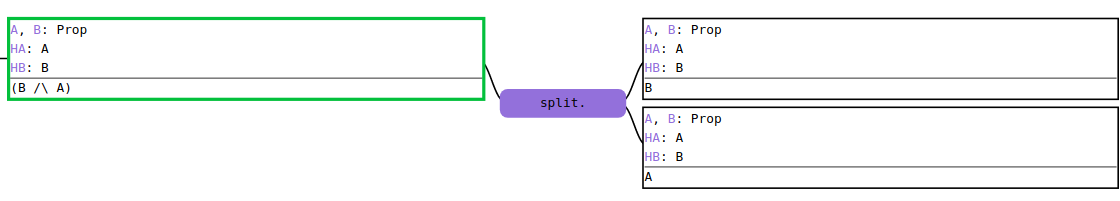
\includegraphics[width=\textwidth]{proof-tree}{\parfillskip=0pt\par}
\caption{Proof-tree view: three obligations nodes and one tactic node}%
\label{proof-tree-view-nodes}
\end{figure*}

When the user enters a proof, a single, root obligation node is created.  This
node corresponds to the current, single proof obligation.  In order to progress,
the user will invoke a tactic.  When they do, a tactic node will be inserted as
a child of the current obligation node, thus denoting that this tactic was ran
from that context.  Depending on the outcome of the tactic execution, one of the
following will happen:

\begin{itemize}

  \item if the tactic yields sub-obligations, these are added as children to the
tactic node, and the focus shifts to the first such sub-obligation,

  \item if the tactic yields no obligation (i.e.\ concludes the current
obligation), then the solved sub-trees are visually folded, and the focus moves
to the next pending obligation, if any.  When there are none, it means the proof
is completed.

\end{itemize}

If the current obligation resulted from the execution of a tactic (i.e. for all
obligations but the root one), the user may backtrack their decision and return
to the state prior to the execution of the parent tactic.


\subsection{Identifying the effects of a tactic: visual diffs}\label{peacoq-design-diffs}

Apart from terminators, which finish an obligation, most tactics will operate a
transformation on the goal of the current context.  The transformations can end
up changing entire types, or replacing sub-terms of some types with other terms.
Some tactics will also add hypotheses, remove some, or reorder hypotheses,
whether voluntarily or as part of how they need to operate.

In order for the user of a proof assistant to assess the usefulness of a
tactic's execution, they must be able to identify what changed by running the
tactic.  This is often done in a ad-hoc way, by going back and forth between the
state before and after the tactic, while visually inspecting differences.  This
is not satisfactory for several reasons.

First, finding out differences using this method is tedious.  Proof contexts
often contain dozens of variables and hypotheses, which makes the task of
finding the changes between two contexts both long, because the user might need
to repeatedly read several lines, and is error-prone, since the user might not
notice a change.

Second, \Coq{} does not offer great facilities for caching results, or viewing
results at a different proof context than the current one.  While rolling back
to the state prior to a tactic's execution is a fairly inexpensive action, due
to the \Coq{}'s state model, going back to the state after the tactic's
execution requires running the tactic again from scratch.  For slow tactics, the
process can be extremely slow, and while the tactic is running, the user might
forget about what they were looking for in the first place.

In order to have a better user experience, one would therefore need to be able
to inspect the state, before and after the execution of a tactic, without having
to run the tactic more than once.  Additionally, visual help indicating which
parts of the context have been modified could help accelerate finding the
effects of a tactic, while reducing the chances of missing a change or
mistakenly spotting a spurious change.

Fortunately, our proof-tree mechanism already provides us with a way of
displaying a before/after view of a proof context with respect to a tactic's
execution.  When a tactic is tried, but not committed to, we can display it as a
child of the current obligation node, and display its result as the child of
this tactic node.  By carefully aligning the two nodes, the user can have an
instant view of the two sides for comparison, without needing to run the tactic
ever again.  We cache those results so that the user can move in the tree
however they want.  Our trees are created in such a way that obligations nodes
have a unique execution history, such that when the user visits the same
obligation node, we can display the same tactic nodes, without needing to run
those tactics again.

We now introduce our notion of \define{visual diffs} as a means to highlight
changes between two proof contexts that are visually juxtaposed.  For a given
hypothesis in the original proof context, one of the following three outcomes
might happen to it as the result of a tactic execution: it may remain the same,
it may disappear, or it may by modified (either by being moved around, of by
having its name, term, or type changed).  Similarly, for a given hypothesis in
the final proof context, it may have originated from an unchanged hypothesis in
the original proof context, from a changed hypothesis in the original proof
context, or it may be a newly introduced hypothesis.

% TODO

\begin{figure*}[!htp]
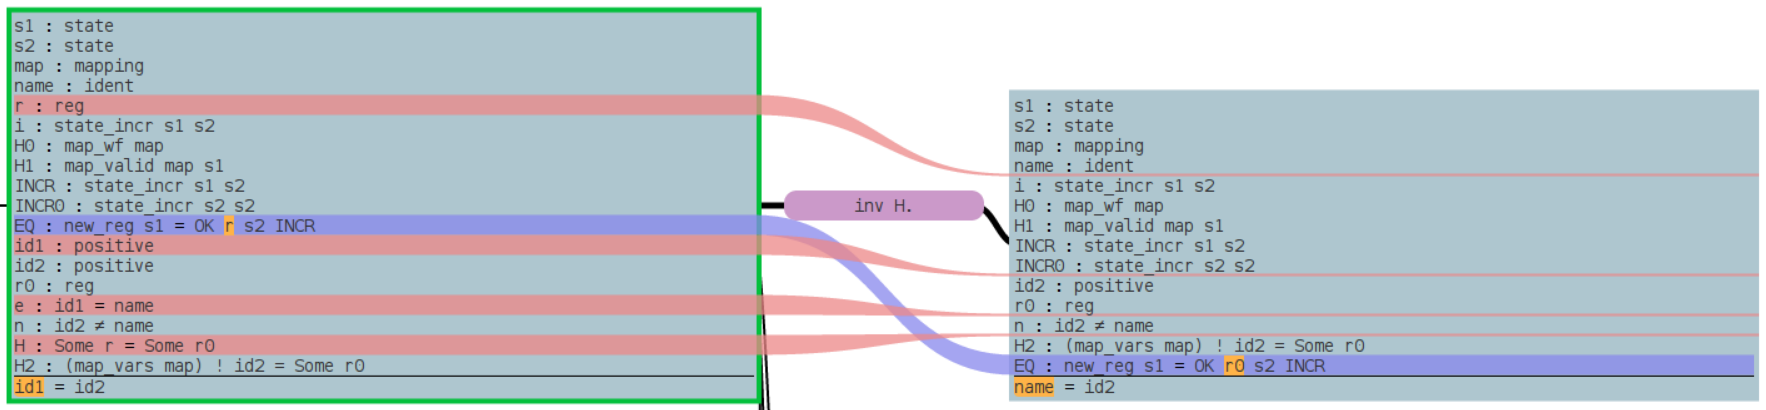
\includegraphics[width=\textwidth]{peacoq-diffs}{\parfillskip=0pt\par}
\caption{Proof-tree visual diff between two obligation nodes}%
\label{proof-tree-diffs}
\end{figure*}


\subsection{Automating tactic exploration in the
background}\label{peacoq-design-automation}

In order to tackle our third identified challenge, that is, helping the user
discover what actions they may take in a given context, we experimented with an
automation technique.  The technique itself is simple: while the user is not
actively entering tactics, we can, in the background, generate and evaluate the
results of a large body of tactics.  We can then estimate which of those tactics
seems relevant to the users and choose how to display them to the user.

The difficulty lies in the details, in particular, we must address the following
problems:

\begin{itemize}

  \item what tactics to try,

  \item which results are relevant,

  \item and how to display those results we deem relevant.

\end{itemize}

We will cover those in order, describing the set of options available.  In our
evaluation, we will highlight which choices we made.

\subsubsection{What tactics to try?}

Because \Coq{} admits \Gallina{} terms as arguments to some \Ltac{} tactics,
there is effectively an infinite number of tactics that can be performed at any
step.  Even ignoring those, many tactics take terms in the environment as
arguments, and the standard library already introduces more than a thousand
terms in the ambient environment.  This makes it clear that an exhaustive search
is not likely.  A couple criteria will help us discern what tactics are worth trying.

First, we can differentiate tactics called \define{terminators} from the ones
that are not.  A terminator is a tactic whose success terminates the current
obligation.  Terminators come in different ways, from very simple ones that find
a proof or a contradiction in the immediate context, to solvers for a given
theory.  For instance, the \coqinline{assumption} tactic is a terminator that
simply looks for an assumption in the current context whose type equates to the
current goal (up to some notion of equality), while the \coqinline{omega} tactic
is a \define{complete} solver for \define{Presburger arithmetic}.  There are
only two outcomes out of the execution of a terminator: either the proof is
found and the tactic succeeds and finishes the current obligation, or its
execution fails.

On the other hand, non-terminator tactics can succeed either by finishing the
current obligation, or by modifying it in any way, or even not doing anything.
They can also lead to the creation of multiple obligations.  For instance, the
\coqinline{split} tactic succeeds on goals that contain a top-level
\define{conjunction}, possibly under a $\Pi$-telescope: it introduces all the
binders in the telescope, and yields two obligations, one for each conjunct.

It is best to test inexpensive terminators first, since a success would mean we
need not look further.  On the other hand, some terminators can effectively
diverge, either by taking an unreasonable amount of time, or by using an
increasingly larger amount of resources, eventually throttling.  In general, we
will need to account for such slowdowns for all tactics with a timeout
mechanism, as we don't want the automation machinery to have a negative
performance impact for our users.

A second important aspect to consider is what arguments to pass to tactics that
require them.  The families of \coqinline{apply} and \coqinline{rewrite}
tactics, for instance, all take as input one term to work with, and, for some, a
second term indicating where to perform the work.  Those terms can either be
variables that are local to the current proof context, or any variable that is
in scope from this file or imported files.  The latter set tends to be between
one and two orders of magnitude larger than the former.  Therefore, while it is
reasonable, but expensive, to try all the proof-local variables, it would be
very expensive to try all identifiers in scope!

\subsubsection{Which results are relevant?}

While we could display all the successful tactics and their outcome to the user,
the amount of information would, in most cases, be overwhelming.  In order for the suggestions to ever be useful, some triage is necessary.

After putting failing tactics out of the picture, one of our first remark is
that many tactics produce the exact same obligations.  Here, one might want to distinguish two close categories:

\begin{itemize}

  \item Two tactics may produce the exact same partial proof term, yielding
equal proof obligations.  This is obviously the case when the two tactics are
aliases of each other, but it can also happen when the two tactics take the same
simple logical step.  Let us refer to those as \define{proof-term equivalent
executions}.

  \item Two tactics may produce the exact same proof obligations (same goals
with same contexts), but build different proof terms.  This could be a concern,
when the terms being built have significant computational differences,
especially in settings where proofs are relevant.  Let us refer to those as
\define{proof-context equivalent executions}.

\end{itemize}

Ideally, we would like to factor out proof-term equivalent executions.  The user
might still care about what tactic is used.  For instance, wherever the
\coqinline{assumption} tactic works, tactics like \coqinline{auto} or
\coqinline{intuition} should also work, but they might do additional work that
is unnecessary.  Similarly, if the assumption being used is called
\coqinline{H}, the tactic \coqinline{exact H} should also work, but it might be
less robust to changes, especially if the name \coqinline{H} was
automatically introduced by \Coq{}.

Finally, the set of tactics available in the \Coq{} proof assistant is not
static: the tactic language is extensible, and users frequently define both
general-purpose and domain-specific tactics.  These can be registered as hints
to the built-in automation mechanism, in which case tactics like
\coqinline{auto} will use them appropriately.  However, as far as we know, at
the current time, there is no built-in mechanism for discovering user-defined
tactics in scope.  An automation mechanism would most likely benefit from such
domain-specific knowledge of tactics to be used in a given proof.

\subsubsection{How to display the relevant results?}

Displaying the outcome of the automation also proves an interesting challenge.
For terminators, or non-terminators that end up solving the current proof
obligation, we can simply indicate to the user that they do.  Tactics that make
progress without solving the proof, however, must be somehow shown to the user
alongside their result.  In the simplest form, one could just present a list of
those tactics, and let the user try them and witness their result on their own.
This imposes quite a bit of cognitive load on the users, as they must visually
inspect one or several proof obligations, trying to understand what changed
between before and after the tactic execution.

To reduce that effort, we benefit from the visualization presented in
Section~\ref{peacoq-design-diffs}.  For each tactic we did not filter out, the
user can align its resulting sub-obligation(s) to the current obligation, and
get visual information about what has changed.

While visual diffs allow the user to quickly inspect the outcome of a given
tactic, if there are too many tactics that make progress, going through them all
one by one can still require a lot of time and concentration.  Some members of
one of our studies indicated the need for grouping the results.  We followed a
static grouping strategy, where tactics were grouped together based on similar
intent: apply tactics, case analysis tactics, rewrite tactics, terminators, etc.
This let users skip over entire classes of tactics that they know are not what
they are currently trying to achieve in the proof.



\section{Evaluation}



\chapter{Assisted refactoring in functional languages}

\chapter{Assisted refactoring in proof assistants}

\chapter{Takeaways}

\appendix

TODO

% Stuff at the end of the dissertation goes in the back matter
\backmatter
\bibliographystyle{plain} % Or whatever style you want like plainnat
\bibliography{references}

\end{document}
